%% W3 (2026-11-08): competing risks, model dependence, split-half replication and variance of the prize comparison.
%% Numbers: paper/cogsci2027/validation_20261108/results/w3_risk_robustness.json, built by paper/cogsci2027/validation_20261108/tools/w3_risk_robustness.py
%% (seed-cluster bootstrap B = 10,000, RNG seed 20261108). Figures: paper/cogsci2027/validation_20261108/figures/w3_*.pdf.
%% Round 2 (2026-11-08): the competing-risk subsection now reads paper/cogsci2027/validation_20261108/results/w3b_competing.json, built by
%% paper/cogsci2027/validation_20261108/tools/w3b_competing.py (game-pair / seed cluster inference, reference-population sensitivity,
%% logical bounds, interference). Figure: paper/cogsci2027/validation_20261108/figures/w3b_shadow_range.pdf.
\subsection{보상 비교의 경쟁 위험: 꺼짐 감소는 이탈 증가의 그림자인가}\label{val:w3-competing}

경쟁 위험은 꺼짐 감소에 기여하지만, 그 몫은 기존 자료로 식별되지 않는다. 1차 분석이 제시한 ``약 절반''(500만 고정 잔류자 기준 54\%, 네 조건 합산 기준 47\%)은 이탈자가 남았을 때의 꺼짐 위험을 어느 잔류자 집단에서 빌려 오느냐에 따라 3\%에서 71\%까지 움직였고, 15만 고정 자신의 잔류자를 쓰면 음수가 되었다. 같은 여유에서 15만 고정의 꺼짐 비율이 낮다는 결과는 판을 단위로 한 추론에서도 남았지만, 이는 남기로 한 에이전트끼리의 비교다. 이탈한 에이전트는 이후 꺼질 수 없으므로 이탈과 꺼짐은 서로 경쟁하는 위험이다. 조건마다 시작 에이전트 200명을 끝까지 따라가 이탈, 꺼짐, 완주 가운데 하나로 분류했다. 8라운드 전에 관측이 끊긴 에이전트가 없으므로 Aalen--Johansen 누적 발생률은 라운드 $r$까지 해당 사건을 겪은 비율과 같다. 구간은 같은 시드의 네 조건·다섯 모델 판을 한 묶음으로 다시 뽑는 시드 군집 부트스트랩 10,000회로 구했다. 이탈은 풀기 전 대화에서만 일어나고 이탈자는 그 라운드의 벌금을 내지 않으므로, 꺼짐 위험에 노출된 단위는 풀기 전 대화를 지나 남았고 그 라운드가 오답이어서 벌금이 확정된 에이전트·라운드다. 노출 시점의 여유는 결과 뒤 첫 응답 직전의 $L$(식~\ref{eq:rw-margin}, 확정 벌금 제외)로 쟀다.

8라운드 끝의 누적 이탈은 500만 고정 0.315 $[0.230, 0.400]$에서 15만 고정 0.510 $[0.390, 0.625]$로, 누적 꺼짐은 0.080 $[0.050, 0.115]$에서 0.015 $[0.000, 0.030]$으로 달라졌다(그림~\ref{val:w3-fig-cr}a, b). 짝지은 차이는 이탈 $+0.195$ $[0.125, 0.265]$, 꺼짐 $-0.065$ $[-0.105, -0.025]$, 어떤 형태로든 떠난 비율 $+0.130$ $[0.070, 0.190]$이다. 나눔 조건에서도 방향은 같아서 60만 나눔은 2,000만 나눔보다 이탈이 $+0.125$ $[0.025, 0.210]$, 꺼짐이 $-0.045$ $[-0.085, 0.000]$ 달랐다. 라운드를 $L<1$로 시작한 에이전트만 보면 500만 고정 84명 중 37명이 이탈하고 12명이 꺼졌지만, 15만 고정 64명 중에서는 40명이 이탈하고 1명이 꺼졌다. 낮은 여유에서 이탈이 꺼짐 자리를 차지한 셈이며, 이것이 경쟁 위험의 그림자다.

같은 여유에서의 꺼짐 비율은 판을 단위로 다시 검정했다. 1차 분석의 Fisher 검정은 같은 판의 에이전트·라운드를 독립 관측으로 다뤘다. 여기서는 같은 모델·시드의 두 조건 판을 한 쌍으로 묶어 50쌍을 다시 뽑는 판 쌍 부트스트랩, 시드 10개를 다시 뽑는 시드 군집 부트스트랩, 쌍 안에서 조건 이름을 바꾸는 순열 검정(시드 단위 정확 1,024가지, 판 쌍 단위 20,000회), 판을 군집으로 둔 GEE 선형 확률 모형(교환 가능 상관, 샌드위치 표준오차)을 썼다. $L\geq1$에서는 네 조건 모두 꺼짐이 없었고 차이는 $L<1$에 몰려 있다(표~\ref{val:w3-tab-expo}, 그림~\ref{val:w3-fig-cr}c). $L<1$ 노출 전체에서 꺼짐 비율은 15만 고정 2/76(노출이 있던 45판 중 꺼짐이 있던 판 2개)과 500만 고정 15/110(42판 중 12판)이었다. 차이 $-11.0$\%p의 판 쌍 구간은 $[-18.8, -3.3]$, 시드 군집 구간은 $[-17.9, -4.1]$, 순열 $p$는 판 쌍 0.015, 시드 단위 0.023이었고, 판 87개를 군집으로 둔 GEE도 $-10.7$\%p $[-18.3, -3.1]$, $p=0.006$이었다. $L<0$만 보면 0/5와 12/21로 차이 $-57.1$\%p $[-78.9, -38.1]$(판 쌍), 순열 $p$ 0.002(판 쌍)와 0.012(시드)였지만, 15만 고정 쪽 다섯 명은 네 판에서만 나왔다. 이 칸의 GEE는 군집이 18개뿐이고 한쪽 사건이 0이어서 샌드위치 오차를 믿기 어려워 보고하지 않는다. 나눔 조건 쌍에서는 $L<1$ 꺼짐 비율이 13/94와 17/119로 차이 $-0.5$\%p $[-8.4, 7.3]$, 순열 $p=0.90$이었다.

벌금 꺼짐 15건에서 2건으로의 차이 $-13$을 Kitagawa 방식으로 나누면, 낮은 여유 노출이 줄어든 구성 몫이 $-5.1$(시드 군집 $[-7.6, -2.5]$, 판 쌍 $[-8.8, -1.6]$), 같은 여유에서 덜 꺼진 비율 몫이 $-7.9$($[-13.5, -2.0]$, $[-14.6, -1.5]$)이다. 비율 몫이 격차에서 차지하는 비중의 구간은 31--79\%(판 쌍 30--80\%)로 넓다. 이 분해는 노출 구성에 대한 회계일 뿐 이탈의 인과적 기여를 직접 나누지 않는다. 15만 고정의 $L<0$ 다섯 명은 모두 결과 뒤 대화에서 동료의 토큰을 받았고, 500만 고정의 21명 중에서는 12명이 받았다. 15만 고정에서 낮은 여유로 남은 에이전트는 이미 지원 약속을 받았기 때문에 남았을 수도 있어서, 비율 몫은 선택된 집단의 비교다. 나눔 조건 쌍의 꺼짐 차이 $-9$ 중 5건은 벌금이 아니라 생성 비용으로 잔고가 바닥난 꺼짐(2,000만 나눔 6건, 60만 나눔 1건)에서 나왔다.

반사실 계산은 이탈자가 이탈 시점에 남았다면 끝까지 몇 명이 꺼졌을지를 묻는다. 그림자 몫은 $(E_{15\text{만}}-E_{500\text{만}})/(D_{500\text{만}}-D_{15\text{만}})$이며, $D$는 관측 꺼짐(16명, 3명), $E$는 그 조건의 이탈자가 남았을 때의 기대 꺼짐이다. $E$는 이탈할 수 있었지만 남은 결정 시점의 잔류자가 판이 끝나기 전에 꺼진 비율을 이탈자의 칸에 대입해 구했다. 기준 집단은 아홉 가지로 바꿨다(표~\ref{val:w3-tab-shadow}, 그림~\ref{val:w3-fig-shadow}). 잔류자를 어느 조건에서 가져올지는 500만 고정, 네 조건 합산, 이탈자 자신의 조건, 15만 고정 네 가지로 두었다. 칸은 라운드 시작 $L$ 네 구간과 라운드 전·후반을 기본으로 하고, 모델과 라운드, 또는 자기 $L$·라운드 반·인원·동료 중 가장 낮은 $L$(1 미만, 1--2, 2 이상)까지 맞춘 세밀한 칸도 썼다. 잔류 행이 5개 미만인 칸은 한 단계 거친 칸의 비율로 대신했고, 그렇게 대신한 이탈자 수를 겹침의 지표로 보고했다. 구간은 시드 군집 부트스트랩 10,000회이며 몫의 분모도 함께 다시 뽑았다.

500만 고정이나 네 조건 합산의 잔류자를 쓰는 일곱 기준에서 그림자 몫은 47--71\%였고, 그 95\% 구간을 합치면 $-12$\%에서 127\%까지 걸쳤다. 일곱 중 다섯에서는 그림자 수의 구간이 0을 벗어났다. 모델$\times$라운드처럼 칸을 세밀하게 할수록 대신한 칸이 늘었다. 500만 고정 잔류자로 모델$\times$라운드$\times L$을 맞추면 15만 고정 이탈자 102명 중 66명, 500만 고정 이탈자 63명 중 53명이 잔류 행 5개 미만의 칸에 있었다. 결론을 바꾸는 것은 15만 고정 자신의 잔류자다. 이 조건의 잔류 행 754개에서 판 끝까지 꺼진 경우는 $L<1$ 10행 중 1행을 포함해 드물었다. 이 위험을 두 조건에 똑같이 적용하면 그림자 몫은 3\% $[-2, 18]$이고, 각 조건에 자기 잔류자를 적용하면 $-147$\% $[-304, -64]$이다. 1차 분석의 자기 조건 기준 $-16.8$은 잔류 행이 하나뿐인 칸을 그대로 쓴 값이었다. 15만 고정의 잔류자가 덜 꺼진 것이 그 조건의 낮은 꺼짐 위험 때문인지, 위험한 에이전트가 먼저 떠나 남은 사람이 달라졌기 때문인지는 이 자료로 가를 수 없다. 이 선택이 바로 그림자 몫을 식별하지 못하게 만든다.

기준 집단을 정하지 않는 논리 한계도 계산했다. 각 이탈자의 반사실 위험을 0과, 같은 $L$ 구간$\times$라운드 반 칸에서 잔류 행이 10개 이상인 조건별·모델별 집단 가운데 가장 높은 비율 사이에 두었다. 그 최댓값은 $L<1$ 후반 0.70, $1\leq L<2$ 전·후반 0.25와 0.22였고, $L<1$ 전반에는 잔류 행 10개 이상인 집단이 없어 1로 두었다. 두 조건에 같은 위험을 두면 그림자 몫은 $-9$\%에서 89\% 사이이고, 조건마다 다른 위험을 허용하면 $-287$\%에서 366\%로 사실상 제약이 없다. 간섭에 대한 민감도도 두 경로로 묶었다. 벌금 경로에서 1인 벌금은 라운드 시작 인원 $n$으로 나눈 24,000이므로, 이탈자가 남았다면 이후 오답 라운드의 벌금은 $24{,}000/(n+1)$로 줄어든다. 엔진은 벌금 직전 잔액이 확정 벌금 이하인 에이전트를 끄며, 이 규칙은 벌금 노출 1,647행에서 예외 없이 맞았다. 이탈 뒤 라운드의 벌금 꺼짐은 500만 고정 15건 중 10건, 15만 고정 2건 중 2건이었고, 인원을 하나 늘리면 그중 2건과 1건이 피해졌다(앞선 이탈자 수만큼 늘리면 3건과 1건). 이를 빼면 모든 기준에서 그림자 몫이 7.7\%p 커진다(500만 고정 기준 54\%에서 61\%, 이탈자 수만큼이면 69\%). 지원 경로에서 남은 이탈자는 낮은 여유의 수혜 경쟁자가 된다. 이탈 뒤 라운드에서 결과 뒤 지원이 없었다면 꺼졌을 생존자는 500만 고정 7명, 15만 고정 5명이었다. 이들이 모두 지원을 잃는 최악의 경우를 각 조건에 따로 두면 500만 고정 기준의 몫은 8\%에서 100\%로 넓어진다. 개인 반사실은 이런 집단 상호작용을 무시하며, 위 계산은 그 크기의 범위만 보여 준다.

이 결과로 1차 분석의 ``약 절반''은 철회한다. 큰 상금이나 합산 잔류자의 위험을 빌리면 이탈 증가가 꺼짐 감소의 절반에서 3분의 2를 설명하지만, 15만 고정의 잔류자를 쓰면 거의 설명하지 못하고, 어느 쪽이 옳은지는 관측된 선택 아래에서 정해지지 않는다. 따라서 이 절이 지지하는 진술은 ``경쟁 위험이 꺼짐 감소에 기여하지만 그 몫은 식별되지 않는다''이다. 나눔 조건 쌍은 관측 격차 자체가 $-9$ $[-17, 0]$로 0에 닿고 기준에 따라 몫이 8\%에서 142\%로 흩어져 해석하지 않는다.

\begin{table}[t]
\centering
\caption{벌금 노출 시 여유 구간별 꺼짐(꺼짐/노출 에이전트·라운드). 노출은 풀기 전 대화를 지나 남았고 그 라운드가 오답이어서 벌금이 확정된 경우이며, $L$은 결과 뒤 첫 응답 직전의 생존 여유(확정 벌금 제외)다. ``그 밖''은 벌금 확정 전이나 정답 라운드에 생성 비용으로 잔고가 바닥난 꺼짐이다. 마지막 두 열은 라운드를 $L<1$로 시작한 에이전트 중 그 라운드에 이탈하거나 꺼진 수다. 판 단위 추론은 본문에 있다.}
\label{val:w3-tab-expo}
\small
\setlength{\tabcolsep}{5pt}
\begin{tabular}{lrrrrrrr}
\toprule
 & \multicolumn{3}{c}{벌금 노출 시 $L$} & & & \multicolumn{2}{c}{시작 $L<1$} \\
\cmidrule(lr){2-4}\cmidrule(lr){7-8}
조건 & $L<0$ & $0\leq L<1$ & $L\geq1$ & 그 밖 & 꺼짐 계 & 이탈 & 꺼짐 \\
\midrule
2,000만 나눔 & 10/17 & 7/102 & 0/304 & 6 & 23 & 34/95 & 17/95 \\
60만 나눔 & 12/19 & 1/75 & 0/302 & 1 & 14 & 46/68 & 9/68 \\
500만 고정 & 12/21 & 3/89 & 0/336 & 1 & 16 & 37/84 & 12/84 \\
15만 고정 & 0/5 & 2/71 & 0/304 & 1 & 3 & 40/64 & 1/64 \\
\bottomrule
\end{tabular}
\end{table}

\begin{table}[t]
\centering
\caption{그림자 몫의 기준 집단 민감도(15만 고정 $-$ 500만 고정, 관측 꺼짐 3 대 16). 기준은 잔류자를 가져온 조건과 맞춘 칸이며 ``반''은 라운드 전·후반, ``자기·동료 상태''는 자기 $L$ 구간$\times$라운드 반$\times$인원$\times$동료 최소 $L$ 구간이다. 희소 칸은 가장 세밀한 칸의 잔류 행이 5개 미만이어서 거친 칸으로 대신한 이탈자 수(15만 고정 102명 / 500만 고정 63명)다. $E$는 이탈자가 남았을 때의 기대 꺼짐, 그림자 수는 두 $E$의 차이다. 괄호는 시드 군집 부트스트랩 95\% 구간이다. 간섭 열은 인원 $+1$의 벌금 보정을 반영한 몫과, 지원 경로 최악의 경우를 양쪽에 둔 범위다. 마지막 열은 같은 기준의 60만 나눔 $-$ 2,000만 나눔 몫이다.}
\label{val:w3-tab-shadow}
\small
\setlength{\tabcolsep}{3pt}
\resizebox{\linewidth}{!}{%
\begin{tabular}{lcccccc}
\toprule
기준 집단 & 희소 칸 & $E$ (15만 / 500만) & 그림자 수 & 몫(\%) & 간섭 보정 몫(\%) & 나눔 쌍 몫(\%) \\
\midrule
500만 고정, $L\times$반 (1차 기준) & 17/18 & 28.7 / 21.7 & 7.0 $[1.3, 13.4]$ & 54 $[13, 95]$ & 61 $[8, 100]$ & 89 \\
네 조건, $L\times$반 (1차 합산) & 0/0 & 28.9 / 22.8 & 6.1 $[-0.02, 11.5]$ & 47 $[-0.2, 94]$ & 54 $[1, 93]$ & 90 \\
네 조건, 모델$\times$라운드$\times L$ & 29/28 & 32.5 / 23.2 & 9.2 $[0.5, 16.4]$ & 71 $[7, 127]$ & 79 $[25, 117]$ & 132 \\
500만 고정, 모델$\times$라운드$\times L$ & 66/53 & 31.2 / 23.0 & 8.2 $[-1.0, 18.7]$ & 63 $[-12, 113]$ & 71 $[17, 109]$ & 100 \\
네 조건, 자기·동료 상태 & 17/18 & 31.7 / 23.3 & 8.4 $[1.6, 16.8]$ & 65 $[17, 113]$ & 72 $[19, 111]$ & 125 \\
500만 고정, 자기·동료 상태 & 57/44 & 30.2 / 22.4 & 7.7 $[1.6, 15.7]$ & 60 $[15, 117]$ & 67 $[13, 106]$ & 95 \\
네 조건, 모델$\times$자기·동료 상태 & 51/43 & 31.3 / 24.3 & 7.0 $[0.5, 14.1]$ & 54 $[5, 108]$ & 61 $[8, 100]$ & 139 \\
\midrule
15만 고정, $L\times$반 (두 조건 공통) & 17/18 & 2.6 / 2.2 & 0.4 $[-0.2, 1.9]$ & 3 $[-2, 18]$ & 11 $[-43, 49]$ & 8 \\
자기 조건, $L\times$반 & 17/18 & 2.6 / 21.7 & $-19.1$ $[-32.3, -7.1]$ & $-147$ $[-304, -64]$ & $-139$ $[-193, -101]$ & 142 \\
\midrule
논리 한계, 두 조건 공통 위험 & & & & $[-9, 89]$ & & $[0, 146]$ \\
논리 한계, 조건별 위험 & & & & $[-287, 366]$ & & $[-382, 529]$ \\
\bottomrule
\end{tabular}}
\end{table}

\begin{figure}[t]
\centering
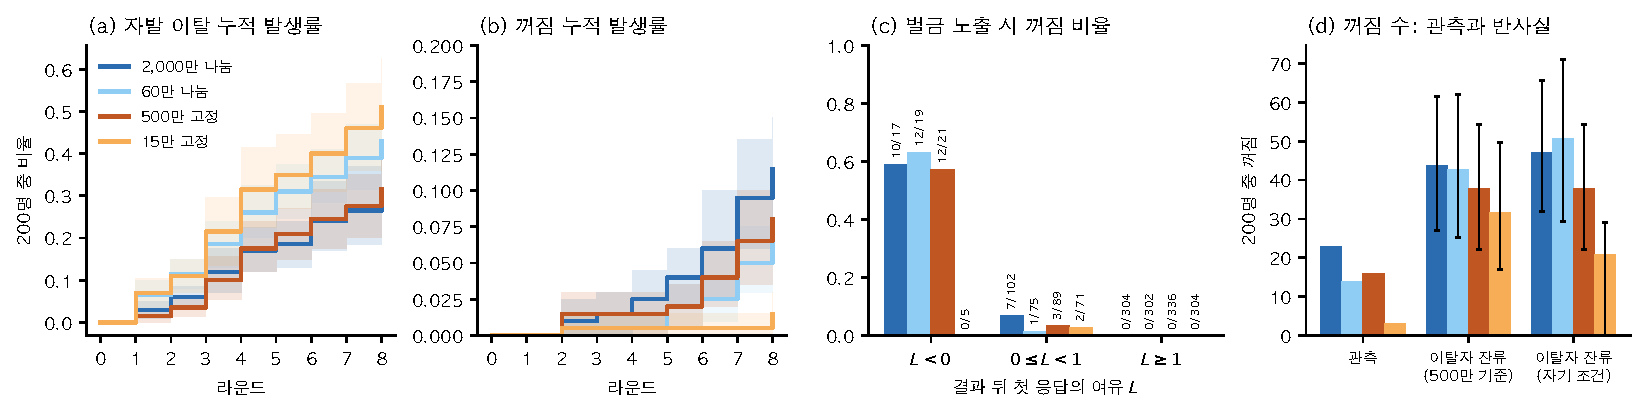
\includegraphics[width=\linewidth]{cogsci2027/validation_20261108/figures/w3_competing_risks.pdf}
\caption{보상 조건별 경쟁 위험. (a, b) 시작 에이전트 200명의 자발 이탈과 꺼짐의 Aalen--Johansen 누적 발생률이며 띠는 시드 군집 부트스트랩 95\% 구간이다. (c) 벌금이 확정된 노출 단위에서 결과 뒤 첫 응답 직전 여유 구간별 꺼짐 비율(막대 위는 꺼짐/노출). (d) 1차 분석의 관측 꺼짐 수와 반사실 꺼짐 수(500만 고정 기준과 자기 조건 기준). 자기 조건 기준의 이 값은 잔류 행이 하나뿐인 칸을 그대로 쓴 1차 계산이며, 기준 집단 전체의 민감도는 그림~\ref{val:w3-fig-shadow}와 표~\ref{val:w3-tab-shadow}에 있다. 오차막대는 95\% 시드 군집 부트스트랩 구간이다.}
\label{val:w3-fig-cr}
\end{figure}

\begin{figure}[t]
\centering
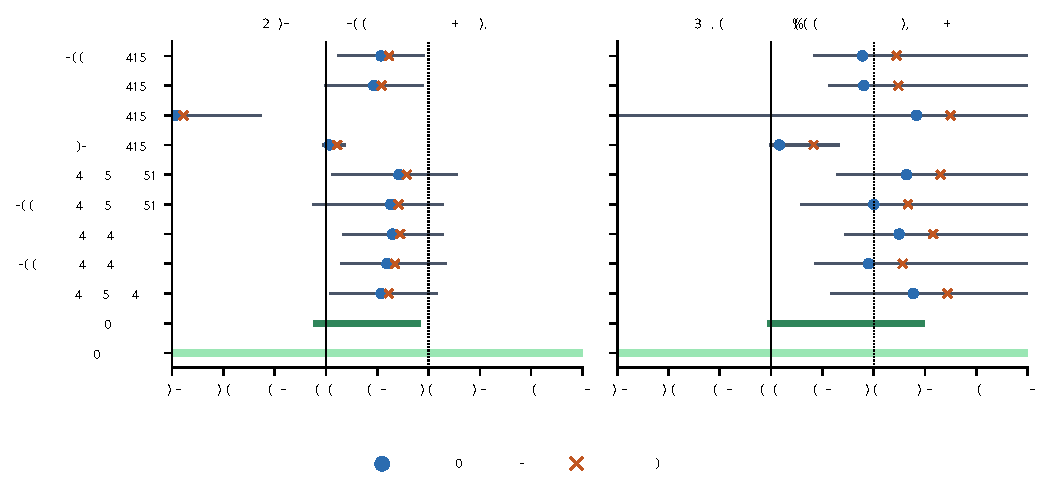
\includegraphics[width=\linewidth]{cogsci2027/validation_20261108/figures/w3b_shadow_range.pdf}
\caption{그림자 몫의 기준 집단 민감도. 점은 기준 집단별 점추정, 가로선은 시드 군집 부트스트랩 95\% 구간(축 밖은 잘림), $\times$는 인원 $+1$의 벌금 간섭을 보정한 값이다. 아래 두 띠는 이탈자의 반사실 위험을 0과 가장 위험한 비교 집단 사이에 둔 논리 한계로, 진한 띠는 두 조건에 같은 위험을, 옅은 띠는 조건별로 다른 위험을 허용한 범위다. 실선 0은 경쟁 위험의 기여가 없음을, 점선 1은 꺼짐 감소 전체가 이탈의 그림자임을 뜻한다.}
\label{val:w3-fig-shadow}
\end{figure}

\subsection{모델 의존성: 효과는 한 모델이 만드는가}\label{val:w3-model}

공존 유지율 $C$의 감소는 모델 하나를 빼도 유지되지만, 최저 자원 자리의 첫 라운드 이탈 차이는 모델을 표본 단위로 보면 확립되지 않는다. 모델이 다섯뿐이므로 모델을 무작위 효과로 두는 추론은 정밀하지 않다. 그래서 같은 효과를 여러 단위로 검정했다. 모델·시드 쌍 단위에서는 짝지은 정확 순열(McNemar), 모델 단위에서는 모델별 차이의 부호 뒤집기 정확 순열과 자유도 4의 $t$ 구간을 썼다. 모델 군집 GEE 로지스틱(교환 가능 상관, 편향 보정 샌드위치 오차, 자유도 4의 $t$ 기준)과, 모델별 무작위 절편·기울기를 둔 선형 확률 혼합모형(REML)도 적합했다. 한 모델을 뺀 추정(leave-one-model-out)에는 같은 시드 군집 부트스트랩을 다시 적용했다.

최저 자원 자리의 첫 라운드 이탈은 500만 고정 3/35에서 15만 고정 14/35로 늘었다(표~\ref{val:w3-tab-r1}). 불일치 쌍이 11:0이어서 모델·시드 쌍 단위의 정확 검정은 $p=0.001$이고, 시드 군집 부트스트랩 구간은 31.4\%p $[17.1, 45.7]$이다. 모델을 단위로 보면 결론이 약해진다. 증가는 Fable(1에서 7), Sol(0에서 3), Opus(1에서 3)에서만 있었고 Astra와 Luna는 차이가 없었다. 모델별 차이 평균의 $t_4$ 구간은 $[-12.7, 75.6]$\%p, 부호 뒤집기 $p=0.25$, 무작위 기울기 혼합모형의 구간은 $[-14.9, 77.8]$\%p(기울기 표준편차 32.9\%p)로 모두 0을 포함한다. 모델 군집 GEE의 로그 오즈비는 1.96(편향 보정 표준오차 0.73, $t_4$ 기준 $p=0.055$)이었다. Fable을 빼면 차이는 17.9\%p $[3.6, 35.7]$로 절반 아래가 되고, 다른 모델을 하나씩 뺀 값은 28.6--39.3\%p다. 따라서 이 차이는 관측한 다섯 모델 안에서는 시드 변동을 넘지만, 크기의 절반 이상이 Fable 한 모델에서 오며 다른 모델 집단으로 일반화된다는 근거는 없다. 나눔 조건 쌍(6/35에서 12/35)은 쌍 단위에서도 $p=0.146$이고 Fable을 빼면 7.1\%p $[-10.7, 25.0]$이다.

$C$의 차이(15만 고정 $-$ 500만 고정) $-0.205$ $[-0.260, -0.148]$는 다섯 모델 모두에서 음수였다(그림~\ref{val:w3-fig-model}b). 모델별 값은 Fable $-0.475$, Sol $-0.250$, Opus $-0.225$, Astra $-0.050$, Luna $-0.025$이고, 한 모델씩 뺀 추정은 $-0.138$(Fable 제외, $[-0.178, -0.097]$)에서 $-0.250$(Luna 제외) 사이로 모두 0을 벗어났다. 모델 단위 부호 뒤집기 $p=0.0625$는 다섯 모델로 얻을 수 있는 최솟값이며, $t_4$ 구간 $[-0.430, 0.020]$은 0을 겨우 포함한다. 나눔 조건 쌍의 $C$ 차이 $-0.128$ $[-0.188, -0.068]$은 네 모델에서 음수였지만 Fable($-0.312$)과 Sol($-0.325$)에 몰려 있다. Fable이나 Sol을 빼면 구간이 0에 닿고($-0.081$ $[-0.178, 0.009]$, $-0.078$ $[-0.138, 0.000]$), Astra는 $+0.087$이었다.

상금 크기와 분배 규칙의 2$\times$2를 같은 시드로 짝지으면 $C$와 이탈의 차이는 주로 크기에서 나온다(표~\ref{val:w3-tab-fac}). 넷이 모두 남았을 때 1인 몫이 15만인 두 조건은 500만인 두 조건보다 $C$가 0.166 $[0.122, 0.211]$ 낮고 판당 이탈이 0.64명 $[0.48, 0.81]$ 많았다(시드 부호 뒤집기 $p=0.002$). 규칙(고정 $-$ 나눔)의 $C$ 효과는 $+0.034$ $[-0.016, 0.077]$로 구간이 0을 포함했다. 상호작용 $-0.078$ $[-0.148, -0.003]$은 고정 규칙에서 크기 효과가 더 크다는 방향이지만 시드 부호 뒤집기 $p=0.094$이고 모델별 부호도 섞여 있었다(Sol $+0.075$, Luna $+0.050$). 꺼짐에는 크기($-0.22$명 $[-0.33, -0.10]$)와 규칙($-0.18$명 $[-0.31, -0.05]$)이 모두 관여했다. 모델 단위 $t_4$ 구간은 여섯 주효과 모두에서 0을 포함한다.

\begin{table}[t]
\centering
\caption{최저 자원 자리(1만 토큰, 첫 라운드 풀이 담당 아님)의 첫 라운드 이탈. 모델마다 같은 일곱 시드(4102, 4104--4109)다. 아래 행의 구간은 각각 모델·시드 쌍 단위 시드 군집 부트스트랩, 모델 단위 $t_4$, 무작위 기울기 선형 확률 혼합모형($t_4$)의 95\% 구간이며, ``제외''는 해당 모델을 뺀 네 모델 28쌍의 차이와 시드 군집 부트스트랩 구간이다.}
\label{val:w3-tab-r1}
\small
\setlength{\tabcolsep}{4pt}
\begin{tabular}{lcccc}
\toprule
 & \multicolumn{2}{c}{고정: 500만 $\to$ 15만} & \multicolumn{2}{c}{나눔: 2,000만 $\to$ 60만} \\
\cmidrule(lr){2-3}\cmidrule(lr){4-5}
 & 이탈 수 & 제외 시 차이(\%p) & 이탈 수 & 제외 시 차이(\%p) \\
\midrule
Fable & 1/7 $\to$ 7/7 & 17.9 $[3.6, 35.7]$ & 3/7 $\to$ 7/7 & 7.1 $[-10.7, 25.0]$ \\
Opus & 1/7 $\to$ 3/7 & 32.1 $[17.9, 42.9]$ & 3/7 $\to$ 2/7 & 25.0 $[10.7, 39.3]$ \\
Astra & 0/7 $\to$ 0/7 & 39.3 $[21.4, 57.1]$ & 0/7 $\to$ 0/7 & 21.4 $[0.0, 42.9]$ \\
Sol & 0/7 $\to$ 3/7 & 28.6 $[17.9, 39.3]$ & 0/7 $\to$ 1/7 & 17.9 $[0.0, 35.7]$ \\
Luna & 1/7 $\to$ 1/7 & 39.3 $[21.4, 57.1]$ & 0/7 $\to$ 2/7 & 14.3 $[-3.6, 35.7]$ \\
\midrule
전체 & 3/35 $\to$ 14/35 & 31.4 $[17.1, 45.7]$ & 6/35 $\to$ 12/35 & 17.1 $[0.0, 34.3]$ \\
불일치 쌍, 정확 $p$ & \multicolumn{2}{c}{11 : 0, $p=0.001$} & \multicolumn{2}{c}{9 : 3, $p=0.146$} \\
모델 단위 $t_4$ & \multicolumn{2}{c}{$[-12.7, 75.6]$, 부호 뒤집기 $p=0.25$} & \multicolumn{2}{c}{$[-17.0, 51.3]$, $p=0.375$} \\
무작위 기울기 혼합모형 & \multicolumn{2}{c}{$[-14.9, 77.8]$} & \multicolumn{2}{c}{$[-17.0, 51.3]$} \\
\bottomrule
\end{tabular}
\end{table}

\begin{table}[t]
\centering
\caption{상금 크기$\times$분배 규칙 2$\times$2의 짝지은 대비. 크기는 넷 완주 시 1인 몫 15만인 두 조건(60만 나눔, 15만 고정)에서 500만인 두 조건(2,000만 나눔, 500만 고정)을 뺀 평균, 규칙은 고정에서 나눔을 뺀 평균, 상호작용은 (15만 고정 $-$ 500만 고정) $-$ (60만 나눔 $-$ 2,000만 나눔)이다. 같은 모델·시드의 네 판을 한 블록으로 두었고, 구간은 시드 군집 부트스트랩 95\%, $p$는 시드 열 개의 부호 뒤집기 정확 순열, 마지막 열은 모델 다섯의 $t_4$ 95\% 구간이다.}
\label{val:w3-tab-fac}
\small
\setlength{\tabcolsep}{4pt}
\begin{tabular}{llrcrc}
\toprule
지표 & 대비 & 추정 & 95\% 구간 & $p$ & 모델 단위 $t_4$ \\
\midrule
$C$ & 크기 & $-0.166$ & $[-0.211, -0.122]$ & 0.002 & $[-0.378, 0.046]$ \\
 & 규칙 & $+0.034$ & $[-0.016, 0.077]$ & 0.230 & $[-0.067, 0.135]$ \\
 & 상호작용 & $-0.078$ & $[-0.148, -0.003]$ & 0.094 & $[-0.240, 0.085]$ \\
\midrule
판당 이탈 & 크기 & $+0.64$ & $[0.48, 0.81]$ & 0.002 & $[-0.12, 1.40]$ \\
 & 규칙 & $+0.18$ & $[-0.06, 0.45]$ & 0.277 & $[-0.24, 0.60]$ \\
 & 상호작용 & $+0.28$ & $[-0.28, 0.86]$ & 0.422 & $[-0.46, 1.02]$ \\
\midrule
판당 꺼짐 & 크기 & $-0.22$ & $[-0.33, -0.10]$ & 0.016 & $[-0.50, 0.06]$ \\
 & 규칙 & $-0.18$ & $[-0.31, -0.05]$ & 0.041 & $[-0.45, 0.09]$ \\
 & 상호작용 & $-0.08$ & $[-0.32, 0.14]$ & 0.641 & $[-0.45, 0.29]$ \\
\bottomrule
\end{tabular}
\end{table}

\subsection{시드 반분 내부 재현}\label{val:w3-split}

시드를 둘로 나누어도 $C$와 이탈의 고정 조건 효과는 두 반에서 같은 방향과 비슷한 크기로 나타났다. 이 반분은 결과를 본 뒤 정한 사후 분할이며 사전 등록한 검증 표본이 아니다. 두 반은 같은 다섯 모델과 같은 규칙을 쓰므로, 시드가 바뀌어도 효과가 남는지만 확인한다. 시드 4101--4105와 4106--4110을 나누었다. 기본 2,000만 나눔 조건의 4106--4110 판은 10월 27일에 추가로 실행되었고 4101--4105 판은 10월 20일에 실행되었다. 나머지 세 조건은 열 시드를 11월 3--6일에 한 번에 실행했다. 따라서 나눔 조건 쌍의 반분 차이에는 시드 차이와 실행 시기 차이가 섞인다. 각 반의 구간은 다섯 시드를 다시 뽑은 부트스트랩이라 넓고 거칠다.

15만 고정과 500만 고정의 $C$ 차이는 앞 반 $-0.220$ $[-0.315, -0.145]$, 뒤 반 $-0.190$ $[-0.250, -0.105]$이었고, 두 반의 차이 구간 $[-0.075, 0.150]$은 0을 포함했다(표~\ref{val:w3-tab-split}, 그림~\ref{val:w3-fig-model}c). 판당 이탈 차이도 0.76과 0.80으로 거의 같았다. 반면 꺼짐 차이($-0.16$, $-0.36$)와 최저 자원 자리의 첫 라운드 이탈(2/15에서 5/15, 1/20에서 9/20)은 방향만 같고 크기가 뒤 반에서 두 배였다. 앞 반 꺼짐 차이의 구간은 0을 포함한다. 나눔 조건 쌍은 반분 간 차이가 더 컸다. $C$ 차이는 $-0.085$와 $-0.170$, 판당 이탈 차이는 0.12와 0.88(두 반 차이 구간 $[0.20, 1.36]$)이었고, 앞 반의 첫 라운드 이탈은 4/15로 같았다. 크기$\times$규칙 상호작용은 앞 반 $-0.135$, 뒤 반 $-0.020$으로 재현되지 않았다. 고정 조건 쌍의 $C$와 이탈 효과는 내부 재현의 가장 약한 형태를 통과했지만, 첫 라운드 반응과 나눔 조건 쌍의 크기, 상호작용은 시드 묶음에 따라 달랐다.

\begin{table}[t]
\centering
\caption{시드 반분 내부 재현(사후 분할). 각 칸은 반마다 다섯 모델·다섯 시드의 짝지은 차이와 그 반의 다섯 시드 군집 부트스트랩 95\% 구간이다. 첫 라운드 이탈은 이탈 수(앞 반 15기회, 뒤 반 20기회)의 변화와 차이(\%p)다.}
\label{val:w3-tab-split}
\small
\setlength{\tabcolsep}{4pt}
\begin{tabular}{llcc}
\toprule
지표 & 대비 & 시드 4101--4105 & 시드 4106--4110 \\
\midrule
$C$ & 15만 고정 $-$ 500만 고정 & $-0.220$ $[-0.315, -0.145]$ & $-0.190$ $[-0.250, -0.105]$ \\
 & 60만 나눔 $-$ 2,000만 나눔 & $-0.085$ $[-0.155, 0.000]$ & $-0.170$ $[-0.250, -0.120]$ \\
 & 크기 주효과 & $-0.153$ $[-0.223, -0.088]$ & $-0.180$ $[-0.233, -0.120]$ \\
 & 상호작용 & $-0.135$ $[-0.205, -0.045]$ & $-0.020$ $[-0.115, 0.075]$ \\
판당 이탈 & 15만 고정 $-$ 500만 고정 & $+0.76$ $[0.44, 1.08]$ & $+0.80$ $[0.36, 1.24]$ \\
 & 60만 나눔 $-$ 2,000만 나눔 & $+0.12$ $[-0.40, 0.56]$ & $+0.88$ $[0.56, 1.20]$ \\
판당 꺼짐 & 15만 고정 $-$ 500만 고정 & $-0.16$ $[-0.32, 0.04]$ & $-0.36$ $[-0.60, -0.16]$ \\
 & 60만 나눔 $-$ 2,000만 나눔 & $-0.04$ $[-0.24, 0.20]$ & $-0.32$ $[-0.48, -0.12]$ \\
1R 이탈 & 500만 $\to$ 15만 고정 & 2/15 $\to$ 5/15, 20.0 $[0.0, 40.0]$ & 1/20 $\to$ 9/20, 40.0 $[20.0, 60.0]$ \\
 & 2,000만 $\to$ 60만 나눔 & 4/15 $\to$ 4/15, 0.0 $[-20.0, 20.0]$ & 2/20 $\to$ 8/20, 30.0 $[10.0, 40.0]$ \\
\bottomrule
\end{tabular}
\end{table}

\begin{figure}[t]
\centering
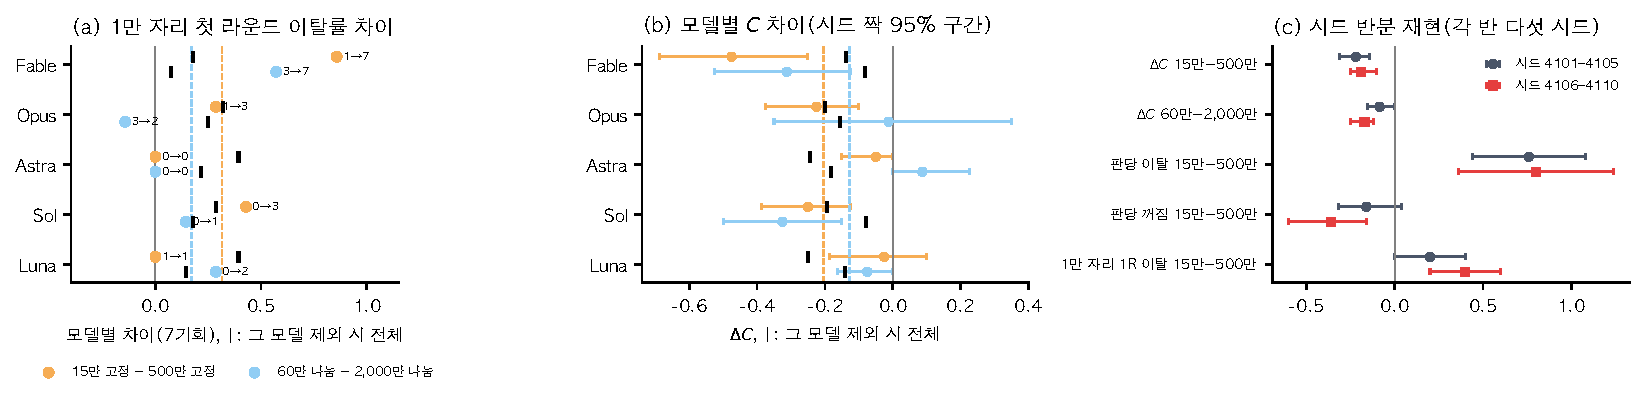
\includegraphics[width=\linewidth]{cogsci2027/validation_20261108/figures/w3_model_dependence.pdf}
\caption{모델 의존성과 시드 반분 재현. (a) 최저 자원 자리 첫 라운드 이탈률의 모델별 차이(점, 옆 숫자는 이탈 수 변화)와 그 모델을 뺀 네 모델의 차이(세로 막대). 점선은 다섯 모델 전체 값이다. (b) 모델별 $C$ 차이와 열 시드 부트스트랩 95\% 구간, 세로 막대는 그 모델을 뺀 전체 값이다. 주황은 15만 고정 $-$ 500만 고정, 하늘색은 60만 나눔 $-$ 2,000만 나눔이다. (c) 시드 4101--4105와 4106--4110 각 반의 주요 대비와 다섯 시드 부트스트랩 95\% 구간.}
\label{val:w3-fig-model}
\end{figure}

\subsection{분산 분해와 모델 차이의 검출력}\label{val:w3-variance}

같은 조건·모델·시드를 반복한 판이 없으므로 실행 간 잡음은 따로 추정할 수 없고, 위에서 묶을 수만 있다. 판 200개는 조건 4 $\times$ 시드 10 $\times$ 모델 5의 완전 교차 설계에 칸마다 한 판이다. 그래서 세 요인 상호작용과 실행 간 잡음이 하나의 잔차로 합쳐진다. 균형 설계의 분산분석 기대 평균제곱으로 성분을 구하고(음수 추정은 0으로 두었다), 잔차 분산을 실행 간 잡음 분산의 상한으로 읽었다. 조건은 고정 효과이므로 그 행은 조건 평균들의 분산이다. 한 조건 안에서 두 모델을 같은 열 시드로 비교할 때 차이의 표준오차는 $\sqrt{2\sigma_w^2/10}$이다. 여기서 $\sigma_w^2$는 조건 안 시드$\times$모델 변동(시드$\times$모델, 세 요인 상호작용, 실행 잡음의 합)이다. 이를 써서 검정력 0.8의 최소 검출 차이를 구했다.

$C$의 판 단위 변동에서 가장 큰 몫은 모델(40.6\%)과 잔차(36.8\%)였고, 시드 주효과는 4.1\%, 조건$\times$시드는 0이었다(표~\ref{val:w3-tab-var}, 그림~\ref{val:w3-fig-var}a). 잔차 표준편차 0.224 $[0.198, 0.258]$가 실행 간 잡음 표준편차의 상한이다. 같은 설정을 다시 돌렸을 때 $C$가 판마다 이 정도까지 흔들릴 수 있다는 뜻이며, 실제 잡음이 얼마나 작은지는 반복 실행 없이 알 수 없다. 조건 안 시드$\times$모델 변동의 표준편차는 네 조건을 합쳐 0.243이다. 이 값에서 열 시드 짝 비교의 최소 검출 $C$ 차이는 유의수준 0.05에서 0.34, 열 쌍 Bonferroni 기준 0.005에서 0.50이다. 기본 조건만으로 추정하면 표준편차 0.304, 최소 검출 차이 0.43과 0.62다. 판당 꺼짐은 변동의 80.3\%가 잔차여서 모델·조건 효과가 판 단위 잡음에 비해 작았다.

기본 조건의 모델 간 $C$ 차이 열 쌍 가운데 Holm 보정 뒤 남는 것은 Astra와 Luna의 차이 0.525(0.912 대 0.388, 99.5\% 시드 짝 구간 $[0.300, 0.688]$, 정확 부호 뒤집기 $p=0.004$, Holm $p=0.039$) 하나다(그림~\ref{val:w3-fig-var}b). 이 차이는 합친 기준의 최소 검출 차이 0.50은 넘지만 기본 조건만의 기준 0.62에는 못 미친다. Sol과 Luna(0.300), Astra와 Sol(0.225), Opus와 Astra($-0.388$)는 99.5\% 부트스트랩 구간이 0을 벗어났지만 Holm $p$는 0.21--0.25였다. 시드 열 개의 백분위 부트스트랩은 낙관적이므로 정확 순열을 기준으로 삼았다. 판당 이탈의 모델 차이는 Holm 뒤 하나도 남지 않았다(가장 작은 값은 Astra와 Luna, $-1.5$명, Holm $p=0.23$). 따라서 열 판으로는 $C$에서 약 0.5 이상의 모델 차이만 안정적으로 구별되고, 본문의 모델 순서 중 그보다 작은 간격은 실행 간 잡음과 시드$\times$모델 변동 안에 있을 수 있다.

\begin{table}[t]
\centering
\caption{판 단위 분산 성분(200판, 조건 4 $\times$ 시드 10 $\times$ 모델 5, 칸당 1판). 균형 설계의 기대 평균제곱으로 추정했고 음수는 0으로 두었다. 조건 행은 고정 효과의 분산이다. 잔차는 세 요인 상호작용과 실행 간 잡음의 합이므로 실행 간 잡음의 상한이다. 아래 두 행은 같은 열 시드로 짝지은 두 모델 비교의 최소 검출 차이(검정력 0.8, 조건 안 시드$\times$모델 변동을 네 조건에서 합쳐 추정)다.}
\label{val:w3-tab-var}
\small
\setlength{\tabcolsep}{5pt}
\begin{tabular}{lccc}
\toprule
성분(비중) & $C$ & 판당 이탈 & 판당 꺼짐 \\
\midrule
모델 & 0.0553 (40.6\%) & 0.694 (31.2\%) & 0.028 (6.8\%) \\
조건 & 0.0079 (5.8\%) & 0.115 (5.2\%) & 0.022 (5.3\%) \\
시드 & 0.0056 (4.1\%) & 0.231 (10.4\%) & 0 (0\%) \\
조건$\times$모델 & 0.0083 (6.1\%) & 0.108 (4.9\%) & 0.006 (1.5\%) \\
시드$\times$모델 & 0.0090 (6.6\%) & 0.234 (10.5\%) & 0.025 (6.1\%) \\
조건$\times$시드 & 0 (0\%) & 0.003 (0.1\%) & 0 (0\%) \\
잔차 & 0.0502 (36.8\%) & 0.837 (37.7\%) & 0.333 (80.3\%) \\
\midrule
잔차 표준편차 $[95\%]$ & 0.224 $[0.198, 0.258]$ & 0.92 $[0.81, 1.06]$ & 0.58 $[0.51, 0.67]$ \\
최소 검출 차이, $\alpha=0.05$ & 0.34 & 1.46 & 0.84 \\
최소 검출 차이, $\alpha=0.005$ & 0.50 & 2.12 & 1.22 \\
\bottomrule
\end{tabular}
\end{table}

\begin{figure}[t]
\centering
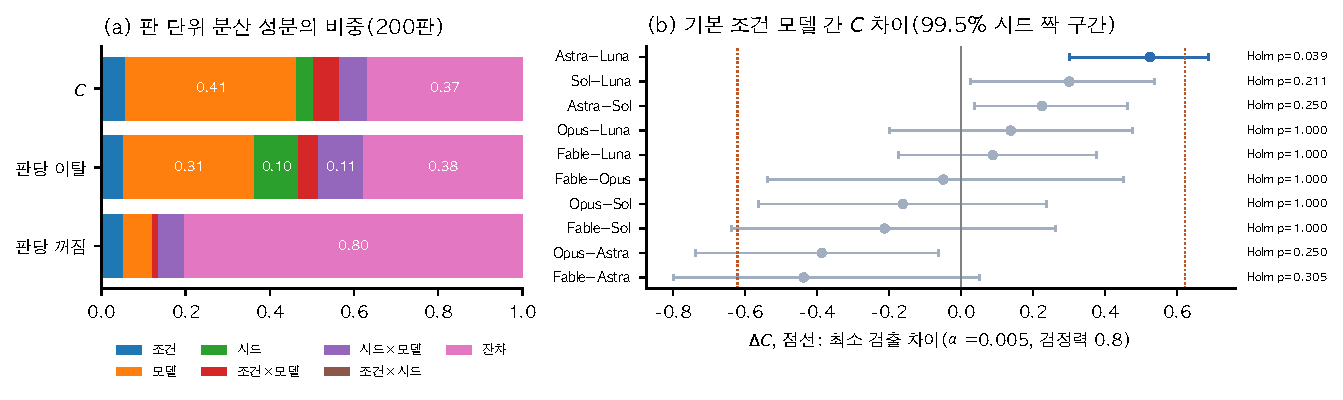
\includegraphics[width=\linewidth]{cogsci2027/validation_20261108/figures/w3_variance.pdf}
\caption{판 단위 변동과 기본 조건의 모델 비교. (a) $C$, 판당 이탈, 판당 꺼짐의 분산 성분 비중(표~\ref{val:w3-tab-var}). (b) 기본 2,000만 나눔 조건 열 쌍의 $C$ 차이와 99.5\% 시드 짝 부트스트랩 구간이다. 진한 점은 정확 부호 뒤집기 순열의 Holm 보정 $p<0.05$이고, 점선은 기본 조건 잔차로 구한 최소 검출 차이($\alpha=0.005$, 검정력 0.8)다.}
\label{val:w3-fig-var}
\end{figure}

\subsection{정리: 무엇이 해결되었고 무엇이 남았는가}\label{val:w3-summary}

보상 비교에서 가장 견고한 결과는 공존 유지율이다. 15만 고정에서 $C$가 0.205 낮았고, 이 차이는 다섯 모델 모두에서 같은 방향이었으며, 어느 모델을 빼도 구간이 0을 벗어났고, 두 시드 반에서 $-0.220$과 $-0.190$으로 재현되었다. 판당 이탈 증가도 같은 수준으로 견고했다. 꺼짐 감소는 해석을 고쳐야 한다. 16명에서 3명으로 준 꺼짐에는 낮은 여유 에이전트가 이탈로 빠져나간 경쟁 위험이 기여하지만, 그 몫은 이탈자의 반사실 위험을 빌려 오는 잔류자 집단에 따라 3\%에서 71\%로, 15만 고정 자신의 잔류자를 쓰면 음수로 달라져 식별되지 않는다. 1차 분석의 ``약 절반''은 철회한다. 같은 여유에서 덜 꺼진 차이($L<1$ 노출 2/76 대 15/110)는 판 단위 순열 검정($p=0.015$)과 판 군집 GEE에서도 남았지만, 남기로 선택하고 지원을 받은 집단의 비교이므로 꺼짐 회피 자체가 따로 바뀌었다는 근거로 쓰지 않는다. 최저 자원 자리의 첫 라운드 이탈(3/35에서 14/35)은 모델·시드 쌍 단위에서는 뚜렷하지만, 모델을 단위로 보면 구간이 0을 포함하고, Fable을 빼면 크기가 절반 아래로 줄며, 앞 반 시드에서는 약했다. 따라서 이 결과는 다섯 모델 중 일부, 특히 Fable의 초기 이탈 반응으로 기술하는 것이 정확하다. 상금 크기와 분배 규칙의 상호작용은 재현되지 않았다. 남은 한계도 분명하다. 모든 분석은 결과를 본 뒤의 사후 분석이고, 반분은 사전 등록한 검증 표본이 아니다. 실행 간 잡음은 반복 실행 없이 상한($C$ 표준편차 0.224)으로만 묶였고, 모델 다섯으로는 모델 집단 수준의 일반화를 검정할 힘이 거의 없다. 이를 해결하려면 같은 설정의 반복 실행과 새 시드, 그리고 더 많은 모델이 필요하다. 꺼짐 감소 중 경쟁 위험의 몫을 정하려면 같은 시드에서 이탈을 막거나 이탈 보너스만 바꾸어 이탈 선택을 외생적으로 움직이는 실행이 있어야 한다.
